\documentclass[11pt,a4paper]{article}
\usepackage[utf8]{inputenc}
\usepackage[margin=2.5cm]{geometry}
\usepackage{amsmath}
\usepackage{siunitx}
\usepackage{booktabs}
\usepackage{pgfplots}
\pgfplotsset{compat=1.17}
\usepackage[hidelinks]{hyperref}

\title{Lab Report 3: The Period of a Simple Pendulum}
\author{Razz \and Omar Haddad}
\date{Physics Laboratory II \\ 22 September 2026}

\begin{document}
\maketitle

\begin{abstract}
We measured the period of a simple pendulum for six lengths between \SI{0.20}{\metre} and \SI{1.20}{\metre}. A linear fit of $T^2$ against $L$ gives a gravitational acceleration of $g = \SI{9.79(6)}{\metre\per\second\squared}$, in agreement with the accepted local value.
\end{abstract}

\section{Theory}

For small amplitudes a pendulum of length $L$ oscillates with period
\begin{equation}
  T = 2\pi \sqrt{\frac{L}{g}},
  \label{eq:period}
\end{equation}
so that $T^2 = (4\pi^2 / g) \, L$. A plot of $T^2$ against $L$ is a straight line through the origin with slope $4\pi^2 / g$.

\section{Method}

A steel bob was hung from a fixed clamp by a light thread. For each length we released the bob from an angle below \ang{10} and timed twenty complete oscillations with a stopwatch, three times. The length was measured from the clamp to the centre of the bob with an uncertainty of \SI{2}{\milli\metre}.

\section{Results}

The measurements are listed in Table~\ref{tab:data} and plotted in Figure~\ref{fig:fit}.

% Mean of three runs of twenty oscillations each.
\begin{table}[ht]
  \centering
  \caption{Measured period for each length.}
  \label{tab:data}
  \begin{tabular}{S[table-format=1.2] S[table-format=2.2] S[table-format=1.3] S[table-format=1.2]}
    \toprule
    {$L$ (\si{\metre})} & {$20T$ (\si{\second})} & {$T$ (\si{\second})} & {$T^2$ (\si{\second\squared})} \\
    \midrule
    0.20 & 18.00 & 0.900 & 0.81 \\
    0.40 & 25.38 & 1.269 & 1.61 \\
    0.60 & 31.18 & 1.559 & 2.43 \\
    0.80 & 35.89 & 1.794 & 3.22 \\
    1.00 & 40.20 & 2.010 & 4.04 \\
    1.20 & 43.95 & 2.198 & 4.83 \\
    \bottomrule
  \end{tabular}
\end{table}


\begin{figure}[ht]
  \centering
  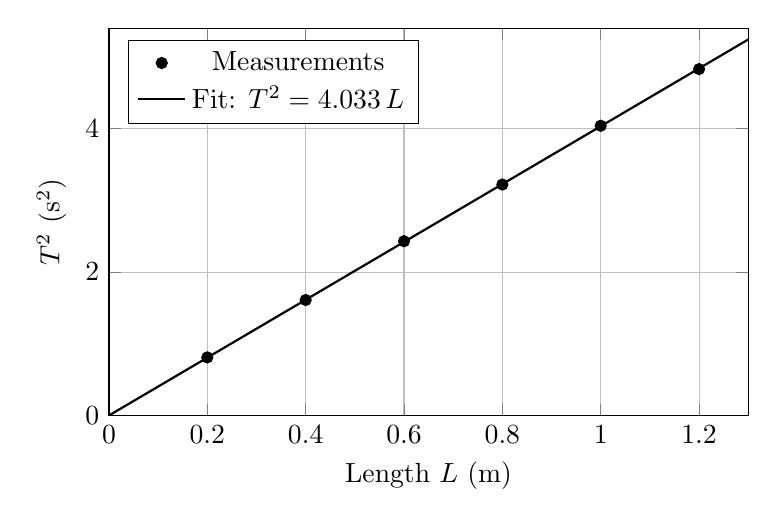
\begin{tikzpicture}
    \begin{axis}[
      width=0.8\textwidth, height=6.5cm,
      xlabel={Length $L$ (\si{\metre})},
      ylabel={$T^2$ (\si{\second\squared})},
      xmin=0, xmax=1.3, ymin=0, ymax=5.4,
      grid=major, legend pos=north west,
    ]
      \addplot[only marks, mark=*, mark size=2pt] coordinates {
        (0.20, 0.81) (0.40, 1.61) (0.60, 2.43) (0.80, 3.22) (1.00, 4.04) (1.20, 4.83)
      };
      \addlegendentry{Measurements}
      \addplot[domain=0:1.3, thick] {4.033 * x};
      \addlegendentry{Fit: $T^2 = 4.033\,L$}
    \end{axis}
  \end{tikzpicture}
  \caption{Squared period against length, with the least-squares line through the origin.}
  \label{fig:fit}
\end{figure}

The fitted slope is \SI{4.033(25)}{\second\squared\per\metre}, which by Equation~\eqref{eq:period} gives
\[
  g = \frac{4\pi^2}{4.033} = \SI{9.79(6)}{\metre\per\second\squared}.
\]

\section{Discussion}

The result agrees with the accepted value of \SI{9.81}{\metre\per\second\squared} within one standard uncertainty. The largest source of error is the reaction time of the person with the stopwatch, about \SI{0.2}{\second} per run, which timing twenty oscillations reduces to \SI{0.01}{\second} per period. The small-angle approximation contributes less than 0.2\% at \ang{10}.

\section{Conclusion}

The period of a simple pendulum is proportional to the square root of its length, as Equation~\eqref{eq:period} predicts, and the measured value of $g$ is consistent with the accepted one.

\end{document}
